\bluepage{Budoucnost OpenGL}

\begin{frame}
\frametitle{OpenGL - budoucnost? - před třemi roky}
	\begin{itemize}
	\item{Zaměří se vývojáři více na OpenGL?}
	\item{Herní společnost Valve vytvořila Linuxovou verzi svého klienta Steam}
	\item{Začala vydávat hry pod Linux - OpenGL}
	\item{Port hry Left4Dead běží rychleji pod Linuxem - pod OpenGL}
	\item{\url{http://blogs.valvesoftware.com/linux/faster-zombies/}}
	\end{itemize}
	\begin{figure}[h]
	
\includegraphics[width=3cm,keepaspectratio]{pics/steam.jpg}
	\end{figure}
\end{frame}

\begin{frame}
\frametitle{OpenGL - Left4Dead - před třemi roky}
	\begin{figure}[h]
	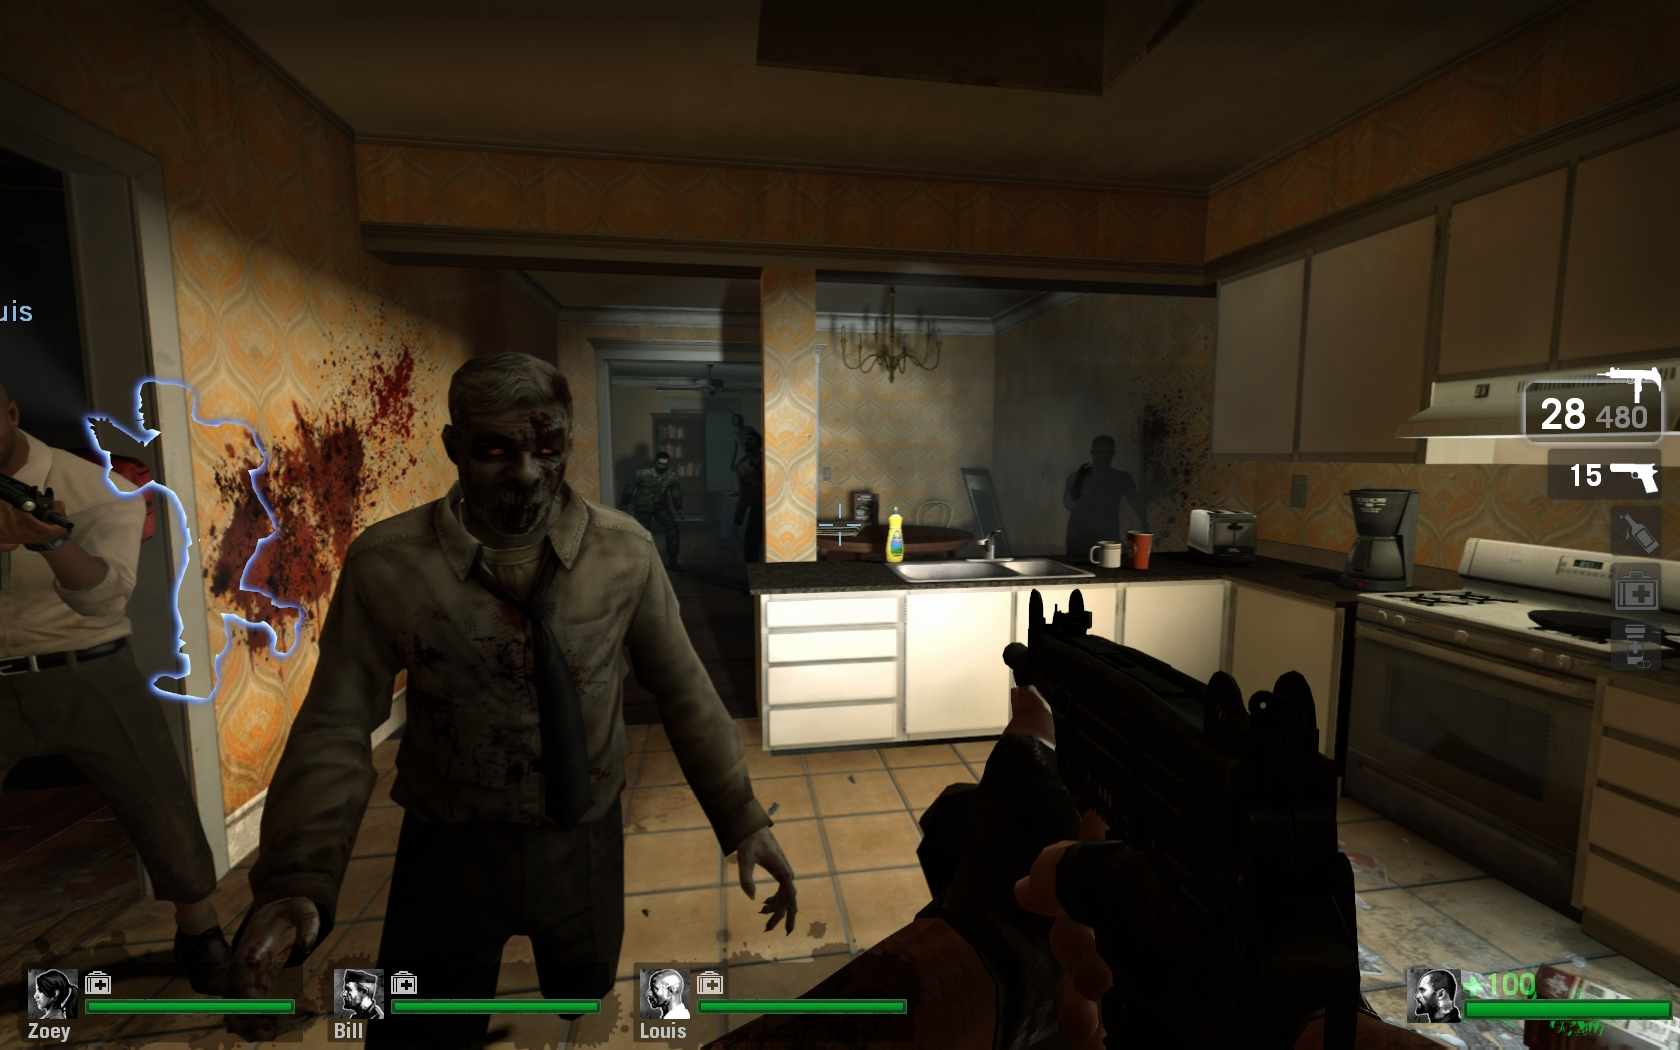
\includegraphics[width=10cm,keepaspectratio]{pics/left4dead.jpg}
	\end{figure}
\end{frame}

\begin{frame}
\frametitle{OpenGL dnes}
  \begin{itemize}
    \item Kolem 2000 her portovaných pod Linux na Steamu
    \item Portování většinou znamená využít SDL + OpenGL
    \item Unity Engine pod Linuxem - OpenGL
    \item Unreal Engine 4 pod Linuxem - OpenGL
    \item Cry Engine 3 pod linuxem - OpenGL
  \end{itemize}
\end{frame}

\begin{frame}
\frametitle{OpenGL budoucnost?}
  \begin{itemize}
    \item Problém spočívá hlavně ve složitosti driverů
    \item Přes 2 milioný řádků kódu pro drivery
    \item OpenGL je poměrně vysokoúrovňové (buffery, schovaná fronta příkazů, synchronizace, ...)
    \item OpenGL je rozsáhlé - přes 800 stran specifikace bez popisu GLSL
    \item Nejednotná mezivrstva jazyka
    \item Kvůli složitost obsahují drivery spousty bugů
    \item Kvůli obecnosti a vysokoúrovňovosti není OpenGL tak rychlé jak by mohlo být (driver overhead)
    \item Vznikla nová specifikace Vulkan a Spir-V
  \end{itemize}
\end{frame}

\begin{frame}
\frametitle{Vulkan}
  \begin{itemize}
    \item Nízkoúrovňové api
    \item Mnohem jednodušší drivery
    \item Jednotná mezivrstva Spir-V, do které se překládají programy (GLSL, OpenCL, ...)
    \item Fronty, command buffer, render passy, shader pipeline, více vláken
    \item Více práce pro aplikační programátory (podobně jako tomu bylo při přechodu na programovatelnou pipeline)
    \item Je pravděpodobné, že bude implementace OpenGL pomocí Vulkan API
  \end{itemize}
	\begin{figure}[h]
	
\includegraphics[width=3cm,keepaspectratio]{pics/vulkan}
	\end{figure}
\end{frame}

